\chapter{O gerador de código}
\label{cap3}

Dada uma especificação na linguagem \TLAA, contendo elementos da lógica TLA e da teoria de conjuntos, além de elementos sintáticos próprios, deseja-se obter uma definição equivalente em linguagem de programação. Equivalência para esse propósito é definida pela igualdade do conjunto de comportamentos permitidos. Isto é, todo comportamento especificado deve ser permitido na execução do código, e todo comportamento permitido pela execução do código deve ter sido especificado.

\section{Elixir}
\label{elixir}

Para esse propósito, a linguagem de programação escolhida para o código traduzido foi Elixir. As motivações são expostas abaixo por ordem de relevância na decisão:
\begin{enumerate}
  \item A concorrência é facilitada por ter seu código traduzido para \textit{bytecode} da máquina virtual do Erlang (BEAM). Suporte a concorrência é de extrema importância, já que \TLA foi criado para facilitar a especificação de sistemas concorrentes. É necessário que o código gerado seja capaz de refletir o sistema também nesse quesito.

  \item Uma linguagem funcional tende a se(setq mouse-wheel-scroll-amount '(1 ((shift) . 1) ((control) . nil)))  aproximar mais de definições matemáticas do que linguagens de outros paradigmas. Uma vez que a estrutura de \TLA foi construída principalmente no âmbito da matemática, a complexidade das traduções tende a ser menor para uma linguagem funcional.

  \item O alto nível de abstração da sintaxe de Elixir, que se inspira em Ruby e sua busca por código facilmente entendível, faz com o programador que trabalhar com o código gerado possa entendê-lo de forma mais simples e rápida do que seria com uma linguagem de baixo nível. Com isso, otimizações podem ser feitas com mais segurança, e a manutenabilidade do código é favorecida.

  \item A transparência de plataforma provida pela máquina virtual BEAM maximiza o número de ambientes aonde o código pode ser executado. Não seria de muito uso gerar um código para um ambiente específico, e uma máquina virtual permite que o código gerado seja \textit{cross plataform}.

  \item O seu código é aberto sobre a licença Apache 2.0, permitindo que o funcionamento de suas estruturas possa ser verificado a qualquer momento. Não seria possível garantir nenhuma correspondência do código gerado com a especificação se não fosse conhecida a execução gerada pelos operadores usados no código.

\end{enumerate}

Essa escolha vem de encontro com a finalidade de proporcionar um código modificável, de forma que o programador seja capaz de entender a correspondência entre as duas partes e minimizando a diferença do nível de abstração no qual ele está programando.

\section{A tradução}
\label{traducao}

A geração de código para uma especificação se dá pela tradução das estruturas de \TLA para Elixir. Esta tradução será feita de forma automática por uma ferramenta escrita em Haskell, implementada durante o corrente trabalho. A ferramenta será responsável pelo \textit{parsing} do aquivo da especificação, no formato \texttt{.tla}, para estruturas internas e, então, transformação dessas estruturas internas em código Elixir.

A escolha da linguagem Haskell para implementação do gerador de código é motivada pela possibilidade da definição de tipos algébricos, que facilitam na representação das estruturas, e na tipagem forte, que ajuda a garantir consistência das relações entre estruturas definidas durante o processo, minimizando a possibilidade de erros no desenvolvimento. Haskell também conta com a biblioteca de \textit{parsing} Parsec, que abstrai a complexidade de analisar sintaticamente um arquivo.

O escopo da tradução se limita à especificação definida, sendo suficiente para gerar código executável para o sistema definido. Traduzir teoremas e suposições não é necessário, uma vez que essas estruturas servem para fazer verificações sobre a especificação e não são necessárias para seu funcionamento. Ao código gerado não é atribuída a responsabilidade de refazer verificações, e sim de manter as propriedades já verificadas.

\subsection{Mapeamentos}
\label{mapeamentos}

A tradução funciona como um grande mapeamento do conjunto de todas as especificações para um conjunto de programas em Elixir. Para viabilizar esse mapeamento, são definidos sub-mapeamentos que traduzem frações de uma especificação. Encontrar sub-mapeamentos suficientes para atender todo o domínio de especificações é suficiente para definir o processo de tradução.

Os primeiros mapeamentos definidos envolvem fórmulas transicionais e variáveis. Para cada fórmula transicional da especificação, é definida uma função, declarada com a sintaxe \texttt{def nome(parametros) do ... end}, que recebe as variáveis como parâmetro. O conjunto de variáveis do sistema é representado em uma Hash - estrutura de dados chave-valor de Elixir, equivalente a um dicionário - representada no padrão \texttt{variaveis = \%\{ variavel1: valor1, variavel2: valor2 \}} e podendo ser acessada com \texttt{variaveis[:variavel1]} para obter \texttt{valor1}.

Cada função mapeada de uma ação recebe uma hash representando o estado atual e retorna outra hash representando o novo estado. O retorno, em Elixir, não exige uma palavra chave - a função retorna aquilo que a última linha retornou, sendo, para as funções geradas, a hash resultante da chamada do seu construtor.

A Figura \ref{fig:esvaziapequeno-elixir} contém a função mapeada da fórmula $EsvaziaPequeno$ definida na Figura \ref{fig:ex1tla}.

\begin{figure}[h]
  \centering
  $\progfig{
  ~~def esvazia\_pequeno(variaveis) do\\
  ~~~~\%\{\\
  ~~~~~~pequeno: 0,\\
  ~~~~~~grande: variaveis[:grande]\\
  ~~~~\}\\
  ~~end
  }$
  \caption{Fórmula transicional $EsvaziaPequeno$ como uma função em Elixir}
\label{fig:esvaziapequeno-elixir}
\end{figure}

Alguns operadores de \TLA permitem mapeamentos ainda mais diretos, como \IF e \CASE, devido a sua inspiração em linguagens de programação. A Figura \ref{fig:pequenoparagrande-elixir} traz a função correspondente à fórmula $PequenoParaGrande$ definida na Figura \ref{fig:ex1tla}. A sintaxe para operadores \IF em Elixir é na forma \texttt{if condição do ... else ... end}.

\begin{figure}[h]
  \centering
  $\progfig{
  ~~def pequeno\_para\_grande(variaveis) do\\
  ~~~~if variaveis[:grande] + variaveis[:pequeno] <= 5 do\\
  ~~~~~~\%\{\\
  ~~~~~~~~pequeno: 0,\\
  ~~~~~~~~grande: variaveis[:grande] + variaveis[:pequeno]\\
  ~~~~~~\}\\
  ~~~~else\\
  ~~~~~~\%\{\\
  ~~~~~~~~pequeno: variaveis[:pequeno] - (5 - variaveis[:grande]),\\
  ~~~~~~~~grande: 5\\
  ~~~~~~\}\\
  ~~~~end\\
  ~~end
  }$
  \caption{Fórmula transicional $PequenoParaGrande$ como uma função em Elixir}
\label{fig:pequenoparagrande-elixir}
\end{figure}

Com o conjunto inicial de mapeamentos apresentado, é possível definir todas as fórmulas transicionais do sistema definido na Seção \ref{exemplo1}. Ao traduzir as definições $Init$ e $Next$, é possível executar concorrentemente todos os comportamentos permitidos pela especificação. A definição $Next$ é traduzida para a função \texttt{main}, que recebe as variáveis para o estado atual e dispara um processo para cada passo permitido por $Next$. Como $Next$ é uma disjunção de todas as ações, é disparado um novo processo com o resultado de cada função traduzida.

Para disparar processos, é chamada a função da biblioteca padrão de Elixir responsável por executar processos ligados: \texttt{spawn\_link}. Essa função é chamada com três parâmetros: o módulo que receberá a chamada, a função a ser executada e uma lista contendo seus parâmetros. Para a tradução de $Next$, o módulo é sempre o módulo do arquivo gerado (\texttt{JarrosDeAgua}), a função é sempre \texttt{main} e os parâmetros são o resultado da aplicação de um dos passos permitidos. O último disparo corresponde à aplicação de um passo balbuciante. A definição dessa função encontra-se na Figura \ref{fig:main-ex1}.

\begin{figure}[h]
  \centering
  $\progfig{
  ~def main(variaveis) do\\
  ~~~spawn\_link JarrosDeAgua, :main, [grande\_para\_pequeno(variaveis)]\\
  ~~~spawn\_link JarrosDeAgua, :main, [pequeno\_para\_grande(variaveis)]\\
  ~~~spawn\_link JarrosDeAgua, :main, [esvazia\_grande(variaveis)]\\
  ~~~spawn\_link JarrosDeAgua, :main, [esvazia\_pequeno(variaveis)]\\
  ~~~spawn\_link JarrosDeAgua, :main, [enche\_grande(variaveis)]\\
  ~~~spawn\_link JarrosDeAgua, :main, [enche\_pequeno(variaveis)]\\
  ~~~spawn\_link JarrosDeAgua, :main, [variaveis]\\
  ~end\\\\
  ~JarrosDeAgua.main(\%\{\ grande: 0, pequeno: 0 \})
  }$
  \caption{Disparo de processos para o sistema de Jarros de Água}
\label{fig:main-ex1}
\end{figure}

A chamada \texttt{JarrosDeAgua.main(\%\{grande: 0, pequeno: 0\})} é a tradução de $Init$. Como esse sistema permite um único estado inicial, apenas uma chamada a \texttt{main} é necessária. Com ela, todos os passos dados para iniciar novos processos terão iniciado com o valor para variáveis que satisfaz a condição inicial. Através da definição de \texttt{main}, é também garantido que todos os passos satisfazem $\square [Next]_{vars}$. Assim, todos os comportamentos iniciados com essa chamada são permitidos por $Spec$, conforme definida na Seção \ref{exemplo1}.

O código gerado para esse sistema não permite, por si só, a solução do problema - uma vez que a especificação não tratava de uma solução. Entretanto, verificou-se que a invariante $jarro\_grande\ \backslash= 4$ não é satisfeita, e portanto um comportamento que leva à solução é permitido por esse sistema. É possível, apenas para fins exploratórios, encontrar os processos disparados pelo código que correspondem a esses comportamentos. Para isso, uma chamada que encerra o programa é invocada se o predicado da invariante for insatisfeito. Essa verificação é feita em todos os passos do comportamento, e portanto é definida como uma condição na função \texttt{main} como na Figura \ref{fig:invariant-ex1}, que imprime os valores das variáveis com \texttt{IO.puts} e encerra o programa com um código de sucesso através de \texttt{:ok}.

\begin{figure}[h]
  \centering
  $\progfig{
  ~def main(variaveis) do\\
  ~~~if variaveis[:grande] == 4 do\\
  ~~~~~IO.puts "\#\{variaveis[:grande]\} \#\{variaveis[:pequeno]\}"\\
  ~~~~~:ok\\
  ~~~end\\
  ~~~\dots\\
  ~end
  }$
  \caption{Exploração de invariantes no código gerado}
\label{fig:invariant-ex1}
\end{figure}

Com essa tradução inicial, é evidenciada a semelhança entre as definições
matemáticas de \TLA e as estruturas do paradigma funcional presentes em Elixir.
Entretanto, o disparo de múltiplos processos contemplando todos os caminhos
possíveis do sistema não é viável dada a explosão de estados nem possui
aplicação prática de muito valor. Assim, se apresenta a maior dificuldade
encontrada durante o deselvolvimento deste trabalho: como traduzir
especificações intermediárias que não descrevem uma implementação e sim um
sistema ou protocolo.

A tradução da especificação completa de uma implementação não resultaria no
disparo de múltiplos processos pela definição $Next$ porque, ao especificar uma
implementação, são definidas quais condições levam a execução de cada ação. Isso
é evidenciado pela comparação das especificações do sistema (Figura
\ref{fig:ex2tla}), do protocolo e da implementação no Capítulo \ref{cap2}. Como o
intuito do gerador de código é fornecer um protótipo funcional e viável, e não
um disparador de processos interminável, são necessárias condições bem definidas
para a decisão de que ação deve ser tomada. A Seção \ref{sec:condicoes}
descreve como a exigência dessas condições é feita.

\subsection{Condições e Ações}
\label{sec:condicoes}

Na definição de uma ação em \TLAA, existem expressões de estado e expressões de
ação (descritas na seção \ref{sec:tla}). As expressões de estado em uma ação
\FANCYA são predicados que terão valoração verdadeira se e somente se o estado em que \FANCYA
será executada - ou seja, o primeiro estado do passo - seja um estado onde
\FANCYA é permitido. Essas expressões, quando dentro da definição de uma ação,
podem ser interpretadas como condições de ativação dessa ação. A ação só pode ser ativada
se suas condições de ativação forem satisfeitas.

Já uma expressão de ação envolve ambos os estados de um passo - o estado atual e
o próximo estado. Se tratada puramente como uma especificação, esse próximo
estado pode ser entendido como qualquer estado possível especificado, de forma
que, de todos os estados possíveis, a expressão de ação só será verdadeira para
aqueles pares de estado que respeitam a condição por ela determinada. Com essa
perspectiva, as expressões de ação também são condições.

Contudo, no contexto de um programa executável viável, os estados são obtidos de
maneira incremental. No código gerado, o estado inicial é obtido pela definicão
do estado inicial da especificação, e os próximos estados são obtidos a partir
da sucessiva aplicação de funções - que representam ações - nesse estado.

Gerar todos os estados possíveis e avaliar uma ``condição de ação'' para cada um dos
passos e então filtrá-los seria uma forma possível de executar o programa, porém
não é viável quando há muitos valores possíveis para as variáveis de estado. Ao
especificar $x' = x + 1$, define-se que todos os pares de estado onde o segundo estado tem o
valor de $x$ igual ao valor $x - 1$ do primeiro estado. Contudo, em uma
implementação, gerar pares de estado que para todos os valores
inteiros e filtrar os que atendem essa condição é
inviável. Nesse contexto, é possível simplesmente gerar os pares de estado válidos e,
considerando que o estado atual é conhecido durante a execução, isso significa apenas
somar 1 ao valor de $x$ para obter o segundo estado do par que satisfaz a ação.

As expressões de ação, no código gerado proposto, são operações efetuadas sobre
um estado que resultam sempre em um novo estado válido. Para isso, elas só são
ativadas quanso as condições de ativação (definidas pelas expressões
de estado) são satisfeitas. A divisão
entre expressões de estado, que serão tranformadas em condições, e expressões de
ação, que serão transformadas em funções que alteram o estado, é feita pelo
próprio parser já que essas expressões se distuinguem na gramática da linguagem
de \TLAA.

Na especificação do protocolo de efetivação em duas fases, na Figura
\ref{fig:ex3tla2}, o tradutor transformará cada uma das ações em duas funções:
uma de retorno booleano determinando se a condição de ativação é satisfeita, e
outra retornando o estado resultante da aplicação da ação.

% exemplo protocolo

\subsection{Determinando a próxima ação}

Como discutido na Seção \ref{sec:protocolo}, a ação de próximo estado $Next$
pode ser atendida por mais de um próximo estado $t$ para o mesmo estado atual $s$.
Isso não é um problema para o TLC, que avalia todos os pares estados possíveis distintos
que atendem as condições da ação, verificando todas as ramificações da árvore de
estados. No programa gerado, contudo, executar uma ação significa fazer possivelmente uma alteração de estado, e
múltiplas alterações de estado não são interessantes para o propósito do
código gerado, conforme discutido na Seção \ref{mapeamentos}.

Assim, é necessário um processo bem definido para decidir qual ação executar a
partir de um estado. Para garantir que seja possível tomar tais decisões sem uma
situação que exija uma escolha, é
necessário que a especificação defina, para cada estado do comportamento, condições de ativação mutualmente
exclusivas para ações disjuntas com próximos estados distintos - isto é,
sempre que há uma disjunção de ações, para todos os estados de um comportamento,
todas as condições de ativação dessas ações devem ser falsas para aquele estado exceto pelas daquelas
que levem ao próximo estado do comportamento.

Uma especificação que atenda essa restrição descreve uma função pura, onde não
há efeitos colaterais e uma mesma entrada, dada pelo estado inicial, sempre gera uma mesma
saída, dada pelo comportamento - sequência de estados - obtido. \TLA permite,
contudo, espeficiar diversos comportamentos válidos a partir do mesmo estado
inicial, o que possibilita que a sequência de estados possa ser eventualmente modificada por
efeitos colaterais e permanecer válida.

Para garantir que o comportamento satisfaz a especificação, as influências de
efeitos colaterais devem obedecer a função de próximo estado. Isso quer dizer
que as influências são, para cada estado da execução, a escolha de uma ação que
satisfaça a função de próximo estado. Como o estado atual $s$ já é conhecido em
tempo de execução, a influência precisa levar a um estado $t$ tal que $<s,t>$
satisfaça tal função.

Quando é definido o conceito de escolha na Seção \ref{sec:protocolo}, define-se que é possível
que exista apenas um valor possível para $t$ que atenda essa restrição. Isso acontece quando a restrição
de condições de ativação mutualmente exclusivas é respeitada pelo estado atual.
Nesse caso, a influência externa não é necessária, já que é possível decidir o
valor de $t$. Assim, a influência externa só é necessária quando uma escolha é
exigida. Nesses casos, o código gerado estabelece uma troca de mensagens entre o
processo gerado pelo modelo e um novo processo denominado oráculo, que será
responsável por toda influência externa no modelo.

\subsection{Concorrência}

Mesmo \TLA sendo uma linguagem de especificação para sistemas concorrentes, ela
não permite descrições para um \textit{fork} ou disparo de novos
processos. O valor de \TLA para sistemas concorrentes é possibilitar um conjunto
de ordens de execução válido, e não limitar a apenas uma única ordem. Sistemas
concorrentes usualmente apresentam muitos comportamentos distintos, e \TLA
permite especificar um modelo que aceite vários desses comportamentos.

Assim, o modelo em si e sua tradução são sequenciais, e se comportam como uma troca
sucessiva de estados. A ordem das transições que alteram esses estados é
possivelmente determinada por uma influência externa - e esta, sim, pode possuir
elementos concorrentes.

Considerando o sistema dos Jarros de Água do Capítulo \ref{cap2}, cada passo da
execução exige uma escolha, já que nenhuma ação tem condição de ativação. Uma
forma de fazer essa escolha é através do disparo de vários processos onde cada
um seleciona uma das possíveis ações - esses procesos podem ser representados
como pessoas com intenções diferentes de resolver o problema dos jarros. Não é
possível permitir que mais de uma pessoa (ou processo) altere o estado dos
jarros ao mesmo tempo. É possível, contudo, a partir de uma fila ou de uma
escolha aleatória de pessoas, estabelecer uma ordem de ações sobre os jarros.

Algumas operações computacionais, como a escrita em um endereço de memória,
serializam ações - já que não podem ser feitos concorrentemente.

A Figura \ref{fig:decide-tla} é um recorte da especificação de transações em
bancos de dados da Figura \ref{fig:ex2tla} e apresenta um exemplo de definição
com expressões de estado e de ação.  

% Primeiro dar exemplo do protocolo e dps vejo o do Decide que é mais complexo

\begin{figure}[h]
  \centering
  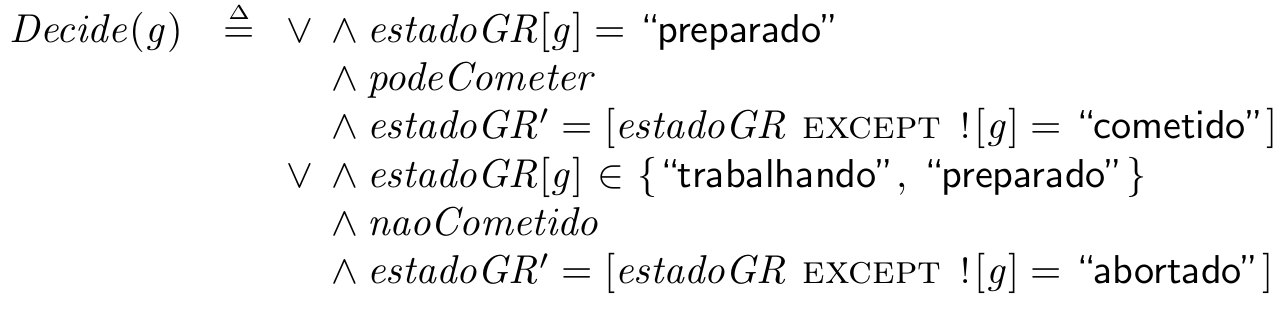
\includegraphics[width=0.8\textwidth]{Decide.png}
  \caption{Especificação de $Decide$ das Transações em bancos de dados}
  \label{fig:decide-tla}
\end{figure}